\documentclass{esannV2}
\usepackage[dvips]{graphicx}
\usepackage[latin1]{inputenc}
\usepackage{amssymb,amsmath,array}
\graphicspath{{images/}}

%***********************************************************************
% !!!! IMPORTANT NOTICE ON TEXT MARGINS !!!!!
%***********************************************************************
%
% Please avoid using DVI2PDF or PS2PDF converters: some undesired
% shifting/scaling may occur when using these programs
% It is strongly recommended to use the DVIPS converters, and to submit
% PS file. You may submit a PDF file if and only if you use ADOBE ACROBAT
% to convert your PS file to PDF.
%
% Check that you have set the paper size to A4 (and NOT to letter) in your
% dvi2ps converter, in Adobe Acrobat if you use it, and in any printer driver
% that you could use.  You also have to disable the 'scale to fit paper' option
% of your printer driver.
%
% In any case, please check carefully that the final size of the top and
% bottom margins is 5.2 cm and of the left and right margins is 4.4 cm.
% It is your responsibility to verify this important requirement.  If these margin requirements and not fulfilled at the end of your file generation process, please use the following commands to correct them.  Otherwise, please do not modify these commands.
%
\voffset 0 cm \hoffset 0 cm \addtolength{\textwidth}{0cm}
\addtolength{\textheight}{0cm}\addtolength{\leftmargin}{0cm}

%***********************************************************************
% !!!! USE OF THE esannV2 LaTeX STYLE FILE !!!!!
%***********************************************************************
%
% Some commands are inserted in the following .tex example file.  Therefore to
% set up your ESANN submission, please use this file and modify it to insert
% your text, rather than staring from a blank .tex file.  In this way, you will
% have the commands inserted in the right place.

\begin{document}
%style file for ESANN manuscripts
\title{LaTeX style file for ESANN manuscripts}

%***********************************************************************
% AUTHORS INFORMATION AREA
%***********************************************************************
\author{Ram\'on H. Mart\'inez-Mayorquin $^1$, Anders Lansner and $^2$ Pawel Herman $^3$
%
% Optional short acknowledgment: remove next line if non-needed
% \thanks{This is an optional funding source acknowledgement.}
%
% DO NOT MODIFY THE FOLLOWING '\vspace' ARGUMENT
\vspace{.3cm}\\
%
% Addresses and institutions (remove "1- " in case of a single institution)
1- KTH - Dept of First Author \\
Address of First Author's school - Country of First Author's
school
%
% Remove the next three lines in case of a single institution
\vspace{.1cm}\\
2- KTH - Dept of Second Author \\
Address of Second Author's school - Country of Second Author's school 
%
\vspace{.1cm}\\
3 School of Second Author - Dept of Second Author \\
Address of Second Author's school - Country of Second Author's school\\ 
}

%***********************************************************************
% END OF AUTHORS INFORMATION AREA
%***********************************************************************

\maketitle

\begin{abstract}
Type your 100 words abstract here. Please do not modify the style
of the paper. In particular, keep the text offsets to zero when
possible (see above in this `ESANNV2.tex' sample file). You may
\emph{slightly} modify it when necessary, but strictly respecting
the margin requirements is mandatory (see the instructions to
authors for more details).
\end{abstract}

\section{Introduction}

This is a sample file. Please use this file to correctly typeset a
submission to the ESANN conference. The associated pdf file will
help you to have an idea of what your paper should look like.

\section{Methods}
The neural network is composed of firing rate units with the following properties. First the individual units receive current from all the other units, that is, the system is a recurrent neural network with all-to-all connectivity. The input current that a unit receives is  is then  thresholded $\theta$ by the logistic function $\Phi(x) = \frac{1}{1 + \exp(-Gx)}$. This whole process is condensed into the equation \ref{eq1}. The input current is then integrated with a time constant $\tau_m$ to determine the activation of the unit. In order to account for the temporal effects we introduce the idea of z-filters that keep information about the activity during a time period $\tau_z$. We can see in equation \ref{eq2} that the filter z follows the activity of the unit at any point in time.

\begin{align}
\tau_m \dfrac{dx_i}{dt} &= \Phi\Big(\sum_{j} W_{ij} z_j - \theta \Big) - x_i \label{eq1} \\ 
\tau_z \dfrac{dz_i}{dt} &= x_i - z_i \label{eq2}
\end{align}

This system allows for the units to keep influencing the other units through $W$ even when they are not longer active. We will see how this property is fundamental for the sequence processing capabilities of our system. 

The connectivity of the system is as depicted in figure \ref{Fig:diagram}. Note that that from each unit emanate two excitatory connections, one that self-reinforces the unit activity $Exc_{self}$ and another that excites the following neuron (contributing to the sequential structure of the activity) $Exc_T$. At the same time every unit inhibits all the units except the next one with $Inh$. Of special relevance are the backwards inhibitory projections that suppress the unit once the next unit in the sequence is activated 

\begin{figure}[h!]
\centering
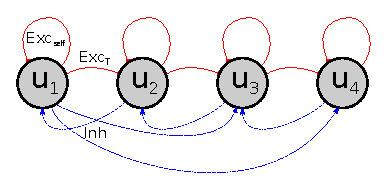
\includegraphics[scale=1.5]{diagram.eps}
\caption{Scheme of the overall network connectivity of the system. Note that the inhibitory connections are only fully depicted for the first unit for the sake of clarity.}\label{Fig:diagram}
\end{figure}

 
\section{Results}

\subsection{The neural network can sustain sequential activity}

In order to recall a particular sequence we cue the first element. This means that we artificially activate the first unit (clamping) of the sequence for a short time. After this initial cue, if the weights have the right configuration, the neural network will continue evolving on its own until the whole particular sequence is correctly recalled as shown in figure  \ref{Fig:recall}.

\begin{figure}[h!]
\centering
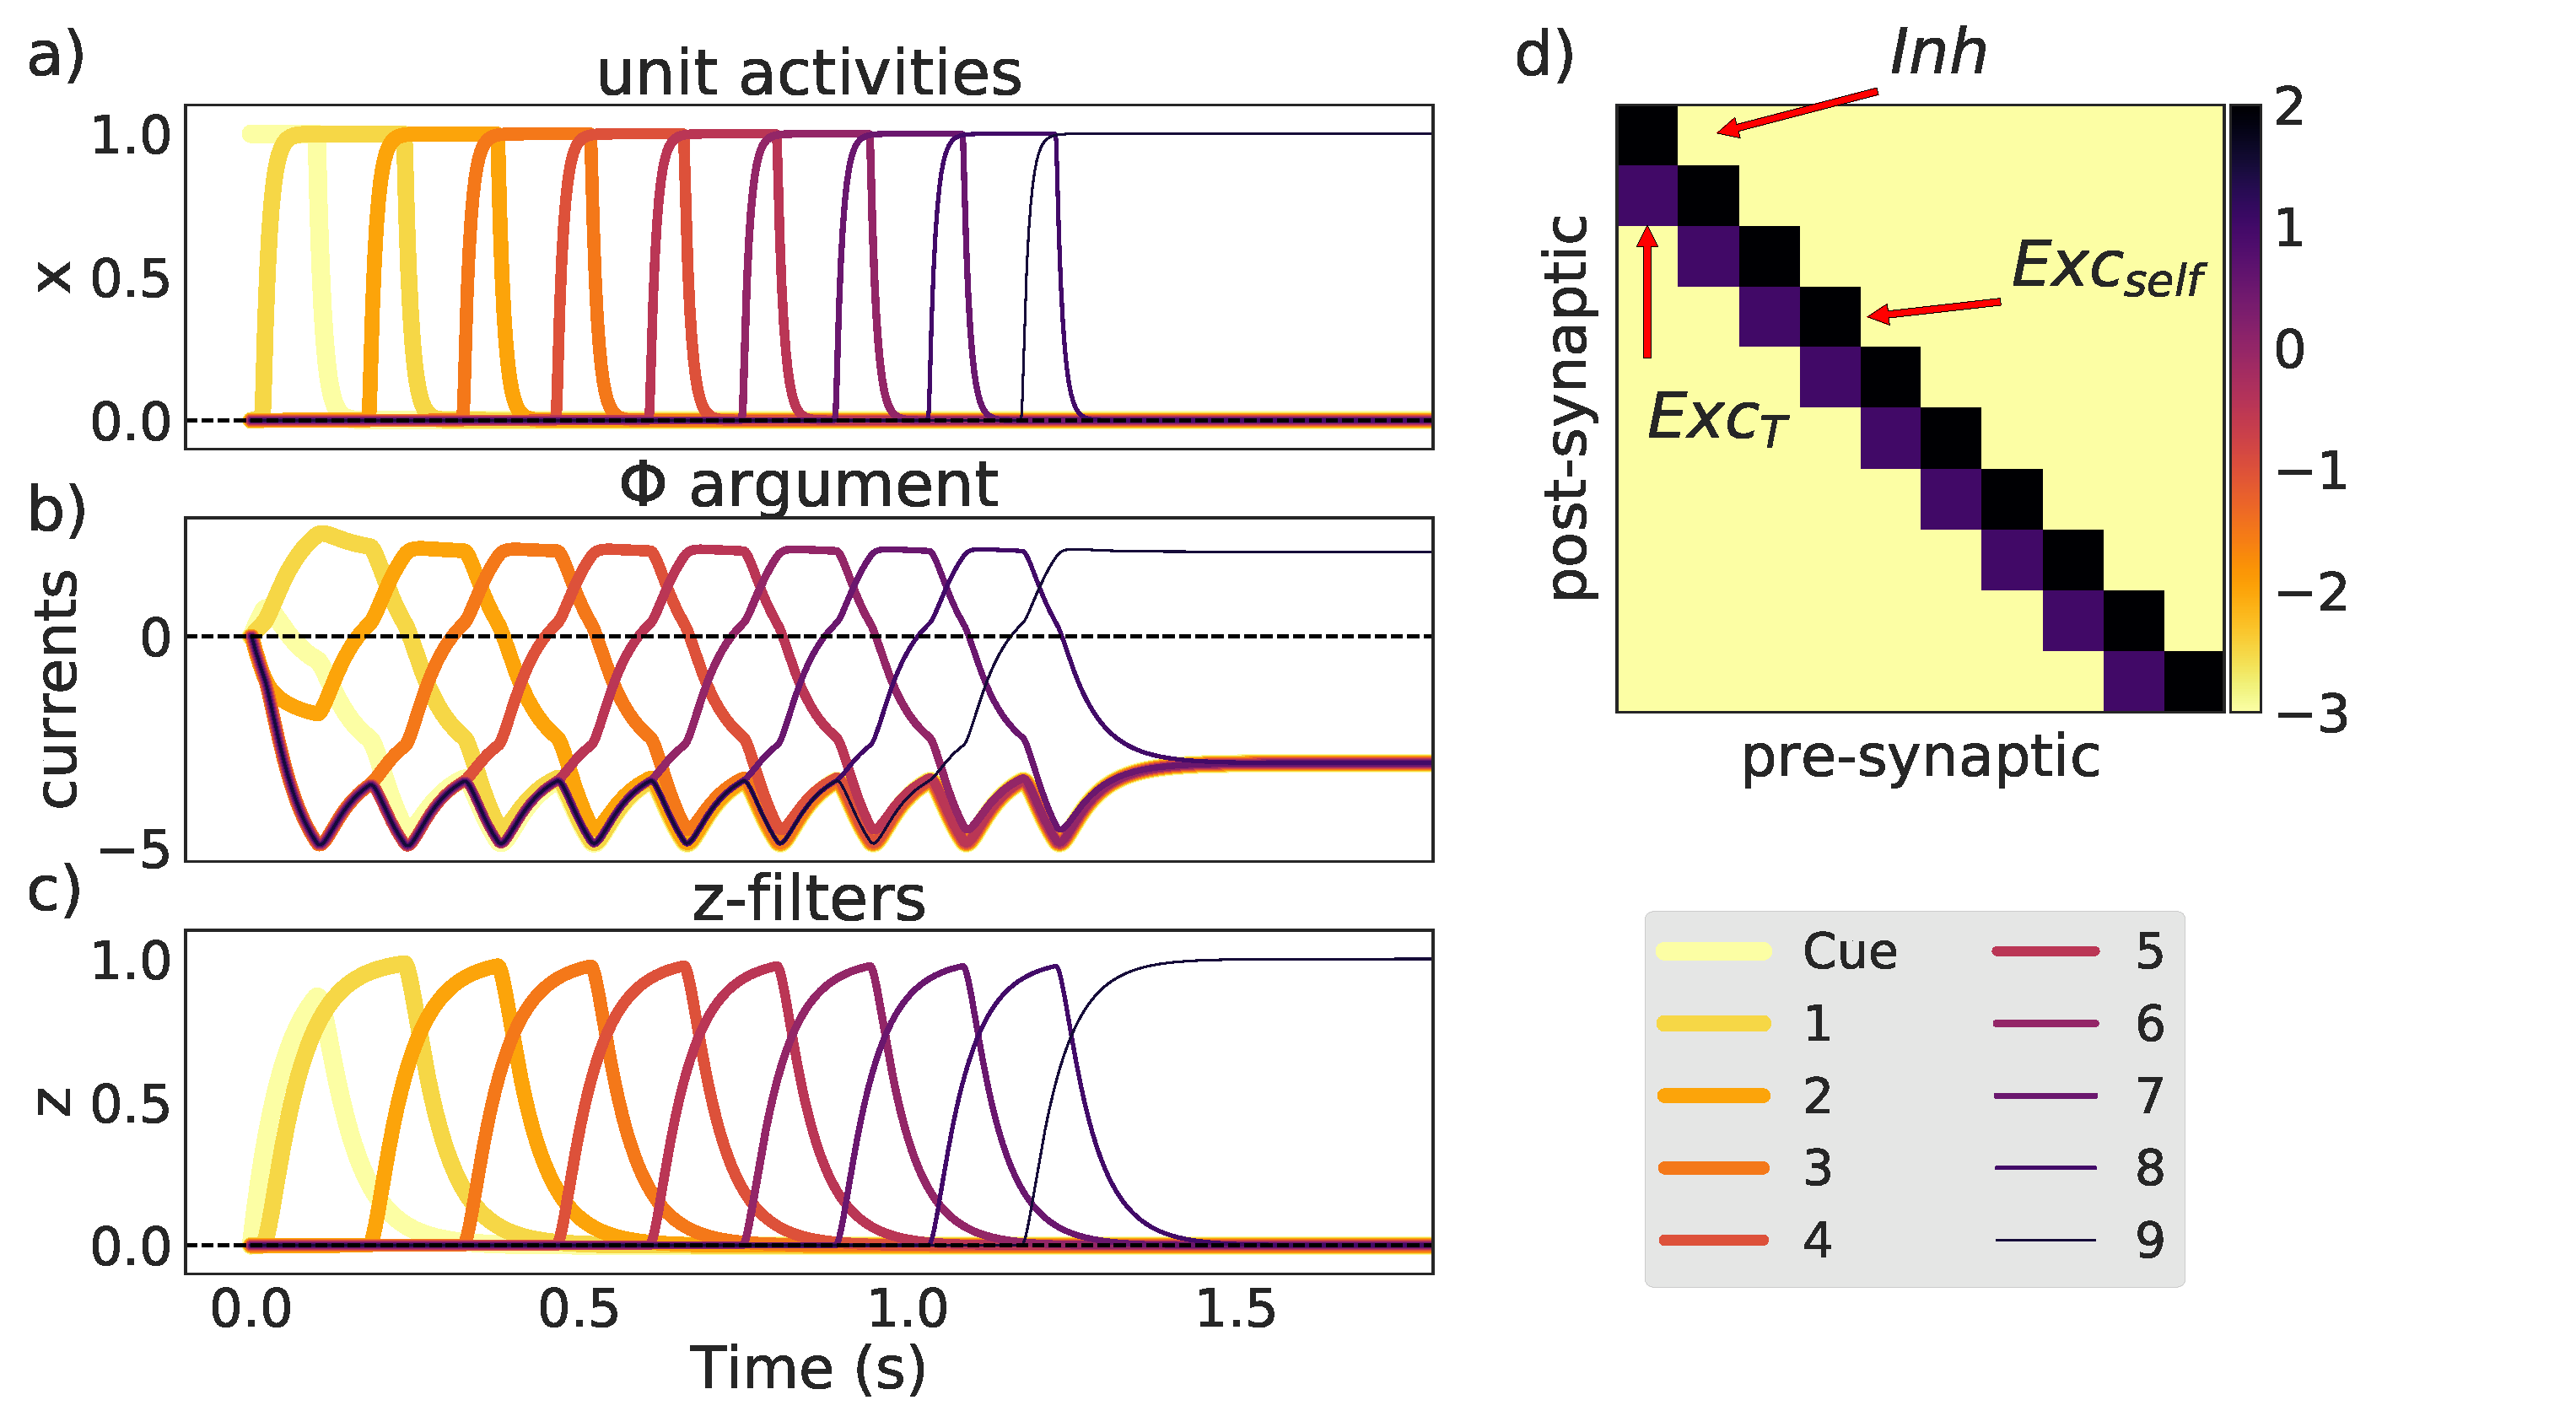
\includegraphics[scale=0.20]{recall.eps}
\caption{Demostration of the successful sequence recall with the corresponding connectivity matrix. a) The activity of the units over time. b) The currents that each unit receives as the sequence progresses. c) the z-filters activations for each unit. d) The connectivity matrix $W$. The weights of the matrix $W$ can be divided into the excitatory connections: the ones on the diagonal that stabilize the unit $Exc_{self}$, the ones under the diagonal that induce transitions $Exc_{T}$ and finally the ones that stabilize the unit  and the inhibitory connections $Inh$ which dominate the matrix $W$. e) The legend with the color codes, we use different colors and thickness to represent the different variables corresponding to different units. }\label{Fig:recall}
\end{figure}

%It is important to note that the weights of the connectivity matrix determine the particular behavior that the network will develop. In the diagonal of the connectivity matrix we have the weights of the excitation connections that keep the unit active once it already became activited $Exc_{self}$. That is, they sustain a positive feed-back loop that keeps the unit active. Below the diagonal, on the other hand, we have the weights of the connections that make the sequence transition from one state to the next $Exc_{T}$. Finally, the rest of the matrix consists of the weights for the inhibitory connections. Of special significance are the backward inhibitory projections above the diagonal, their role is to suppress the last pattern of the sequence once the next unit is activated. 

It is now instructive to detail at the level of the dynamics how the sequential activity is propagated. After the first unit $x_1$ has been activated for long enough due to clamping the filter $z_1$ will start catching up with the activity by increasing its value. It follow then that the unit corresponding to $x_2$ will receive a growing current with value $Exc_{T} \times z_1$ because of the forward connectivity. As this process continues there will be a point in time (exactly at $Exc_{T}(1 - e^{-\frac{t}{\tau_z}}) - \theta = 0$) when $x_2$ will receive enough current to become activated. This in turn will prompt the filter $z_2$ to start catching up initializing the describe process again. On the other hand as soon as the second filter starts growing $z_2$ the first unit will start receiving an inhibitory current $Inh \times z_2$ due to the backward inhibitory projection, this will in turn suppress the unit $x_1$ allowing the sequence to propagate. Finally, once the unit $x_1$ is finally suppressed the excitatory current mediated by $Exc_T$ will be diminished which in most cases would also suppress the activity of $x_2$ if were not for the self-sustaining current $Exc_{self} \times z_2$. In short, the term $Exc_T$ ensures the transition of the activity from one unit of the sequence to the next whereas the competition between $Exc_{self}$ and $Inh$ first lock the pattern unit and then finally suppress it allowing the sequence to evolve towards its end without hindrance.

With the knowledge above in mind we can envision the following  failure scenarios for the sequential dynamics. First, if the magnitude of $Exc_{self}$ is small the self-excitatory current will not be big enough to overcome the threshold and the sequence will not propagate. Second, if $Exc_{Self}$ is big enough to keep the unit active but $Exc_{T}$ is not big enough the next unit in the sequence will not be activated and the sequence will not propagate, in this case we are stuck in the first pattern forever. If both $Exc_{self}$ is big enough to sustain the activity and $Exc_{T}$ is big enough to propagate it but the inhibitory connection $Inh$ is not big enough to suppress the units the result will be that all the units in the sequence will be activated at the end. 


\subsection{The neural network possess a wide dynamic range}

A common problem in sequence learning is to scale the time duration of the sequence according to the needs of the context. In terms of a neural network it means that once the dynamics of sequence recalling are stored in the shape of the weights we can control the \textit{recall time} of the sequence with the internal parameters of the network where we define the recall time as the amount of time that a particular unit is active during a sequence retrieval. In our network there are a two parameters that a priori are strong candidates to regulate the recall time: the transition weight $Exc_T$ by controlling how fast you activate the next unit in the sequence and the threshold $\theta$ by controlling how long it takes for the current to activate the next unit in a sequence. Here we show the exact results for $Exc_T$ but the reasoning for $\theta$ is analogous.  

In order to calculate the recall time we make the following consideration. Once the unit $x_1$ becomes activated the filter $z_1$ starts increasing its value and the unit $x_2$ will be receiving an excitatory current $Exc_T \times z_1$. The point in time $t_{recall}$ at which the this current overcomes the threshold will be the recall time. Using that reasoning we can solve the following equation to calculate the recall time: $Exc_{T}(1 - e^{-\frac{t}{\tau_z}}) - \theta = 0$. If we do we end up with the following expression: $T_{recall} = \tau_z \log(\frac{Exc_T}{Exc_T - \theta})$. This expression tells us that we actually have a singularity at $Exc_T = \theta$, which for our purposes means that can make the recall time arbitrarily by setting this two parameters close enough. In our neural network however, there are more currents into play because of the all-to-all connectivity, we can include those corrections and we end up with an expression of the form $T_{recall} = \tau_z \log(\frac{Exc_T + Inh}{Exc_T - \theta})$ which also possess the after-mentioned property. We can see an illustration of the wide dynamical range of our system in figure \ref{Fig:dynamical_range} where we also show two examples of sequence recall with different $Exc_T$ values and therefore with different recall times. 



\begin{figure}[h!]
\centering
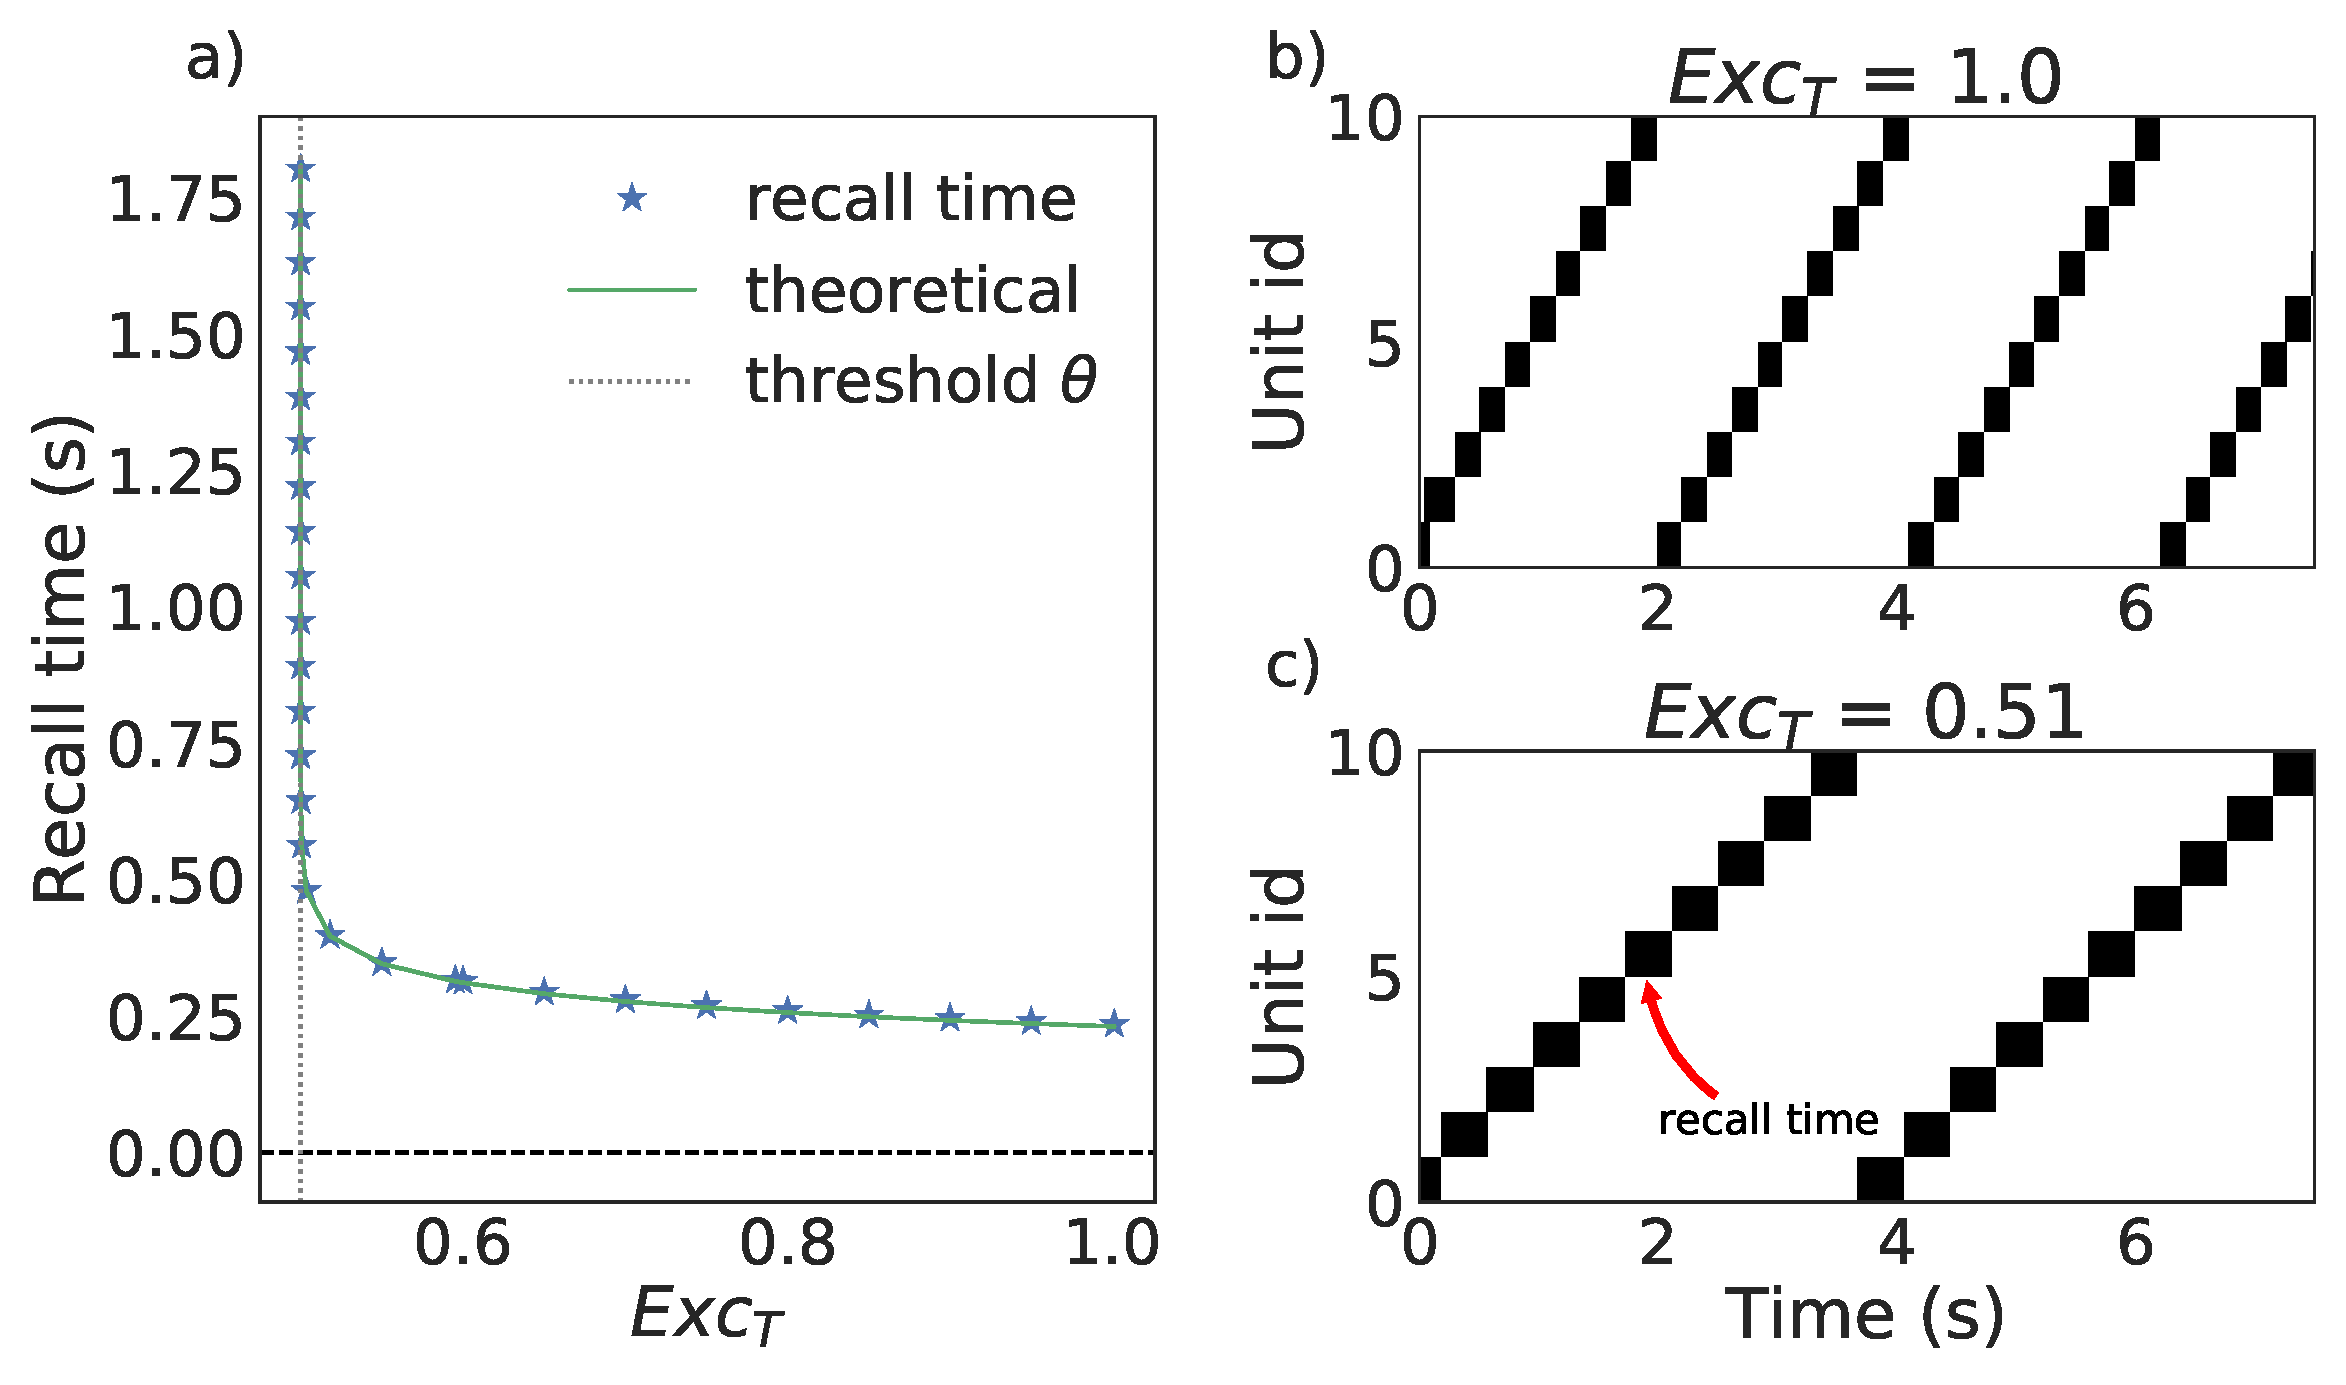
\includegraphics[scale=0.25]{dynamical_range.eps}
\caption{The network posses a wide dynamical range. a) Here we compare the calculated thoretical expression with simulations with our network for different values of $Exc_T$. Note the singularity at $\theta$. b) The network activity with a short recall time. c) The network activity with a longer recall time ($Exc_T$ close to $\theta$).}\label{Fig:dynamical_range}
\end{figure}



\subsection{Learning Rule}
Here we present a learning rule that allows the system to self-organize in the presence of sequential activity, that is, we can equip our network with the capability to learn how to reproduce sequences. We present a learning rule in the equations bellow. The first term is completly hebbian \cite{hebb2005organization} and its role is to strength the connections between units that are activate together. However, in this case, we use the z-filters instead of the activities directly which allow us to bend units in time. We include here another filter like the one in equation \ref{eq2} but with a shorter time constant $\tau_{z_{post}}$. The second term is called synaptic gating \cite{andrew2003spiking} and it allow us to create inhibitory connections when two units are not activated together. We introduce two different variations of this term to explore the functional implications of both. Finally both terms are saturated by maximal and minimal values $w_{max}$ and $w_{min}$. 

\begin{align}
\tag{pre-synaptic}
\tau_w \dfrac{dw}{dt} &= (w_{max} - w) z_{pre}z_{post} + (w_{min} - w) (1 - z_{post})z_{pre} \label{eq:pre-synaptic rule}  \\
\tag{post-synaptic}
\tau_w \dfrac{dw}{dt} &= \underbrace{(w_{max} - w)}_{\text{saturation}} \underbrace{z_{pre}z_{post}}_{\text{Hebbian}} + \underbrace{(w_{min} - w)}_{\text{saturation}}\underbrace{ (1 - z_{pre})z_{post}}_{\text{synaptic-gating}} \label{eq:post-synaptic rule}
\end{align}

The nature and the role of both the hebbian and the synaptic gating terms are better explained in the diagram shown in figure \ref{Fig:plasticity diagram}. There we can appreciate the the main difference between the two rules is on whether they produce a negative contribution when either $z_{pre}$ and $z_{post}$ is activated. In figure \ref{Fig:epochs} we illustrate the results of the training rule

\begin{figure}[h!]
\centering
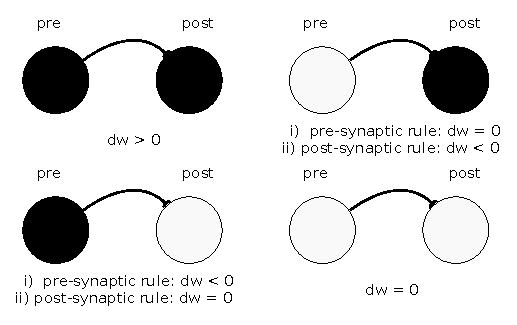
\includegraphics[scale=1.3]{plasticity_diagram.eps}
\caption{Conceptual illustration of the mechanism of learning induced synaptic changes. Here the a black filling stands for an active unit a) Hebbian associative plasticity that implies a weight increase when both pre- and pos-synaptic units are simultaneously active b) In the case of the post-synaptic rule the weight is decreased if the post-synaptic unit itself active without the pre-synaptic unit being active. c) In the case of the pre-synaptic rule the weight is decreased if the pre-synaptic unit is itself active without the post-synaptic unit being active. d) If neither pre- nor post-synaptic units are active, there is no weight modification.}\label{Fig:plasticity diagram}
\end{figure}


\begin{figure}[h!]
\centering
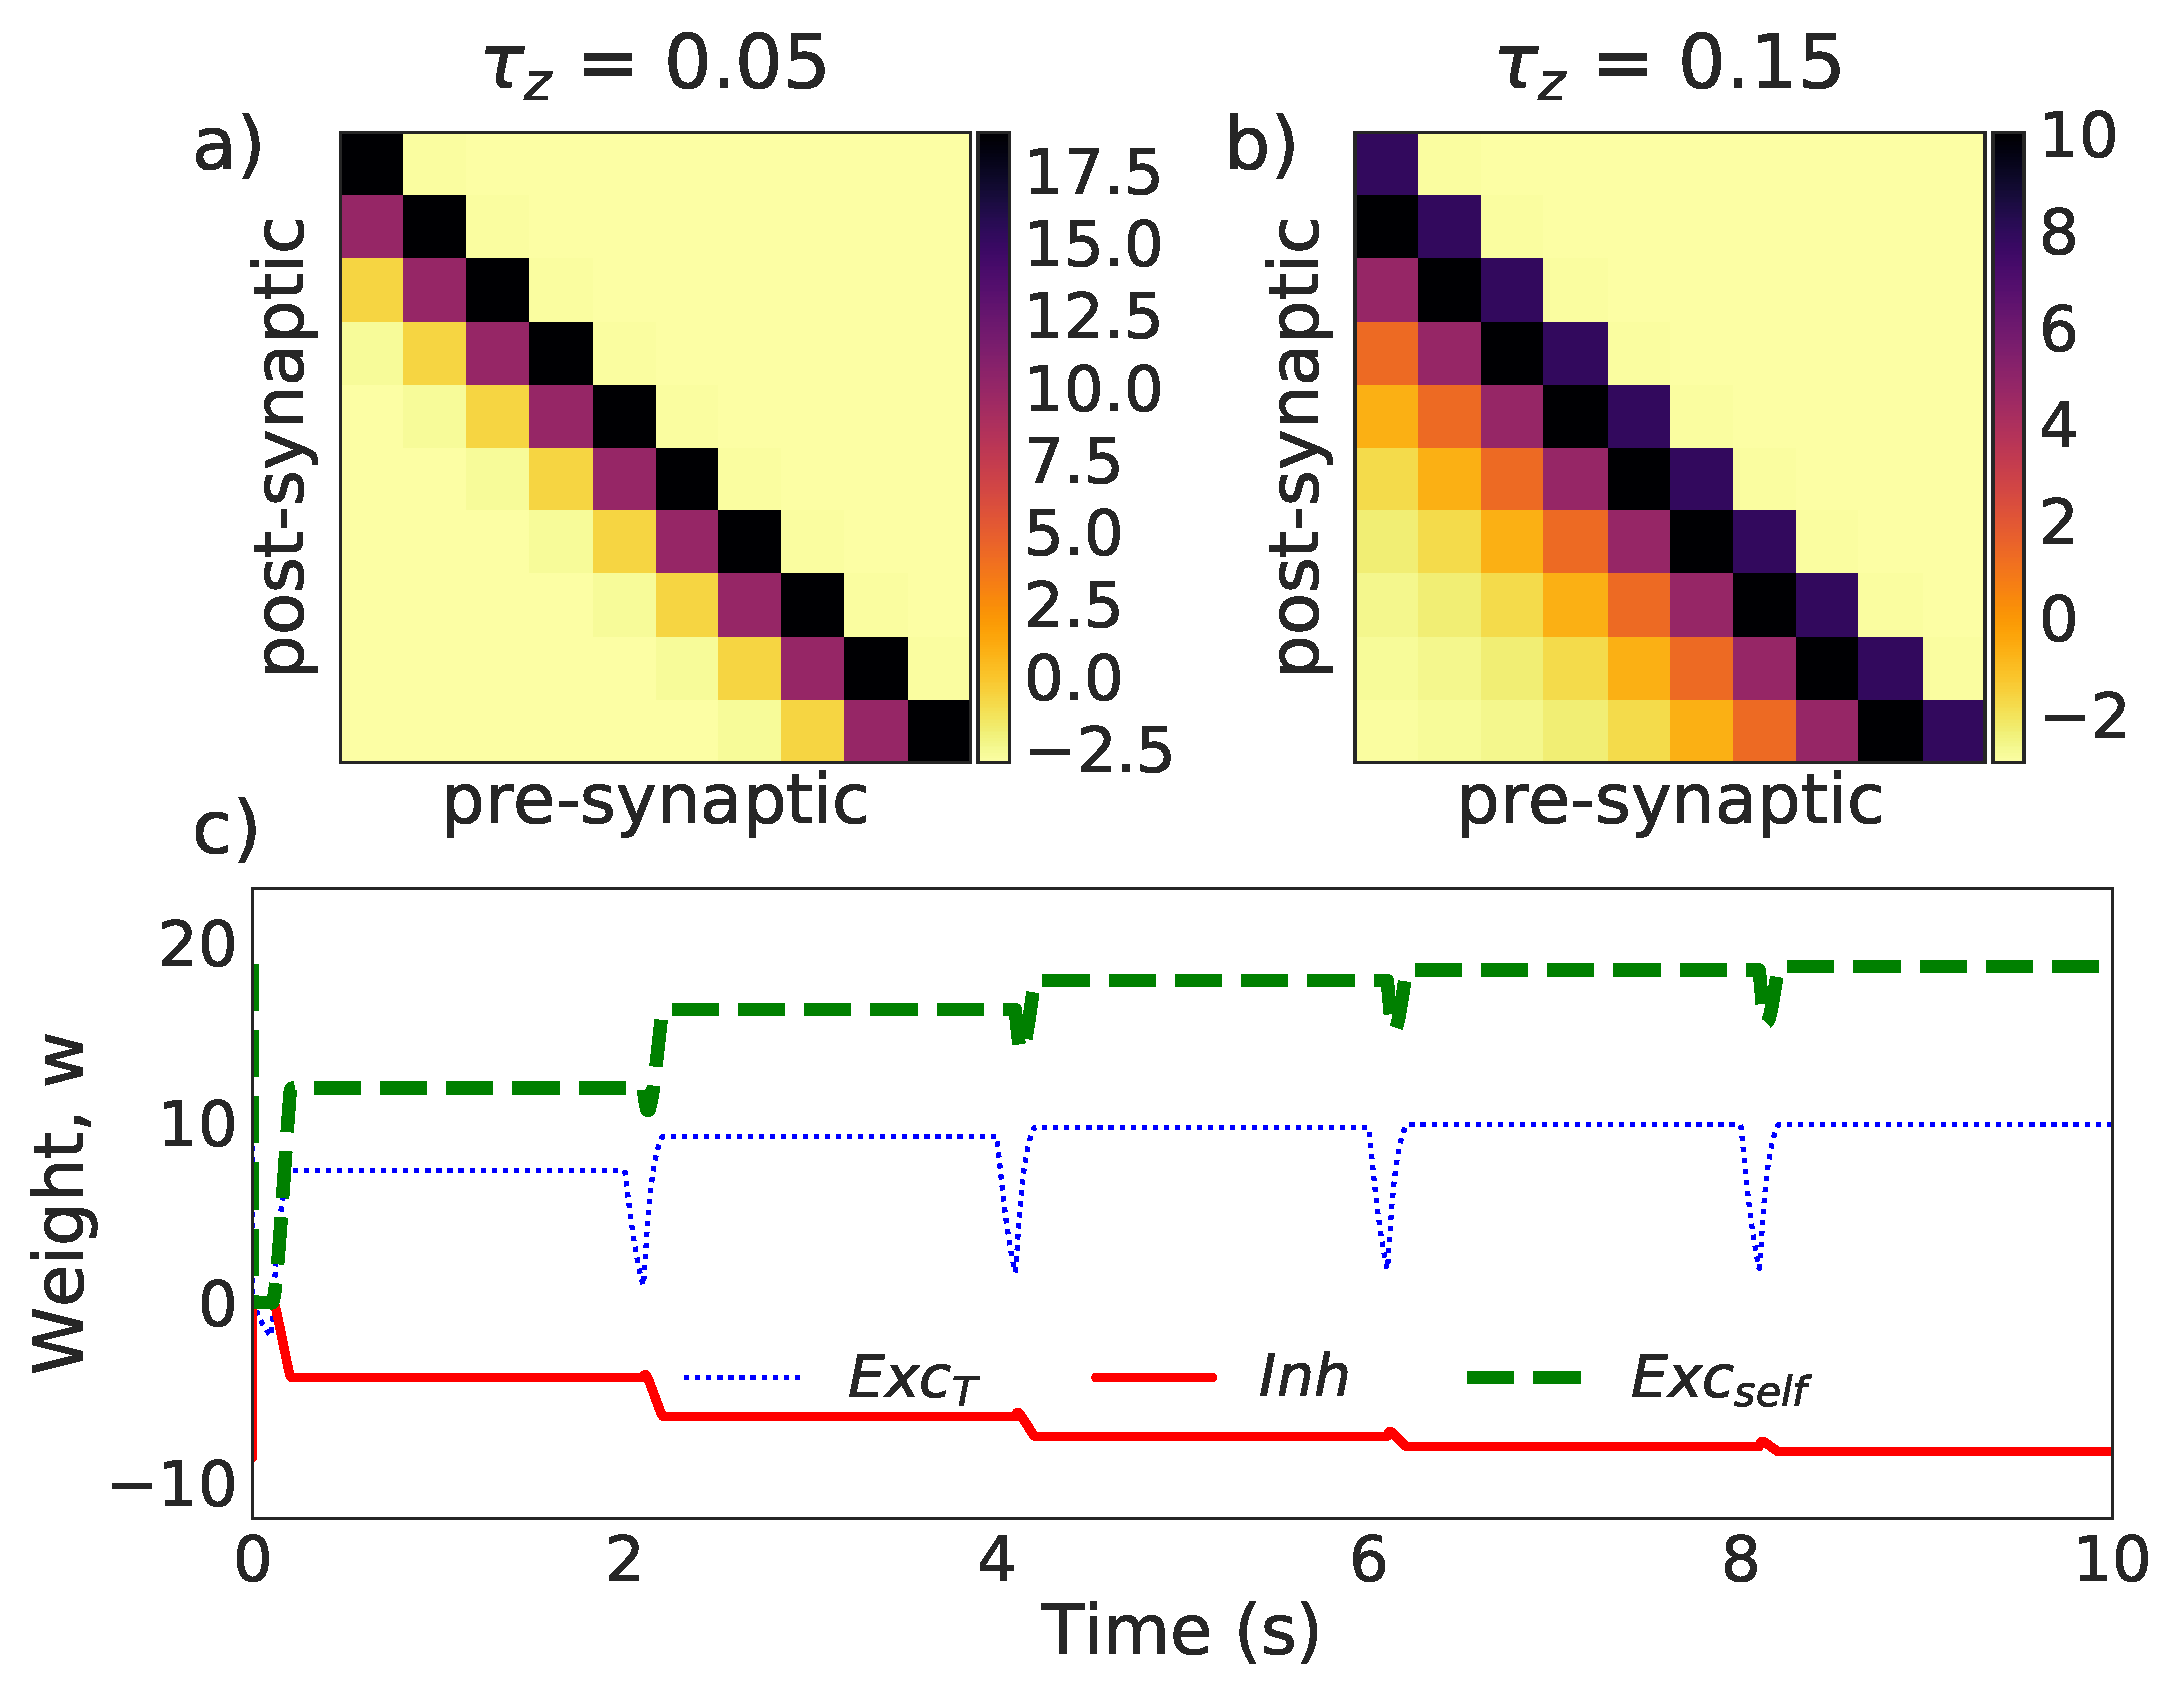
\includegraphics[scale=0.3]{training_rule.eps}
\caption{The effect of training with the learning rule. a) An example of training with a small value of $tau_z=0.050s$. b) Same procedure as in a but with a longer time constant $\tau_z=0.150s$. c) evolution in time of the connection weights from the first to the second unit $Exc_T$, the one from the second back to the first unit $Inh$ and finally of the second unit into itself $Exc_{self}$. Five epochs of length $2s$ are shown here, note that this is enough time for the weights to stabilize.}\label{Fig:epochs}
\end{figure}



\subsubsection{Learning rule and control}


\begin{figure}[h!]
\centering
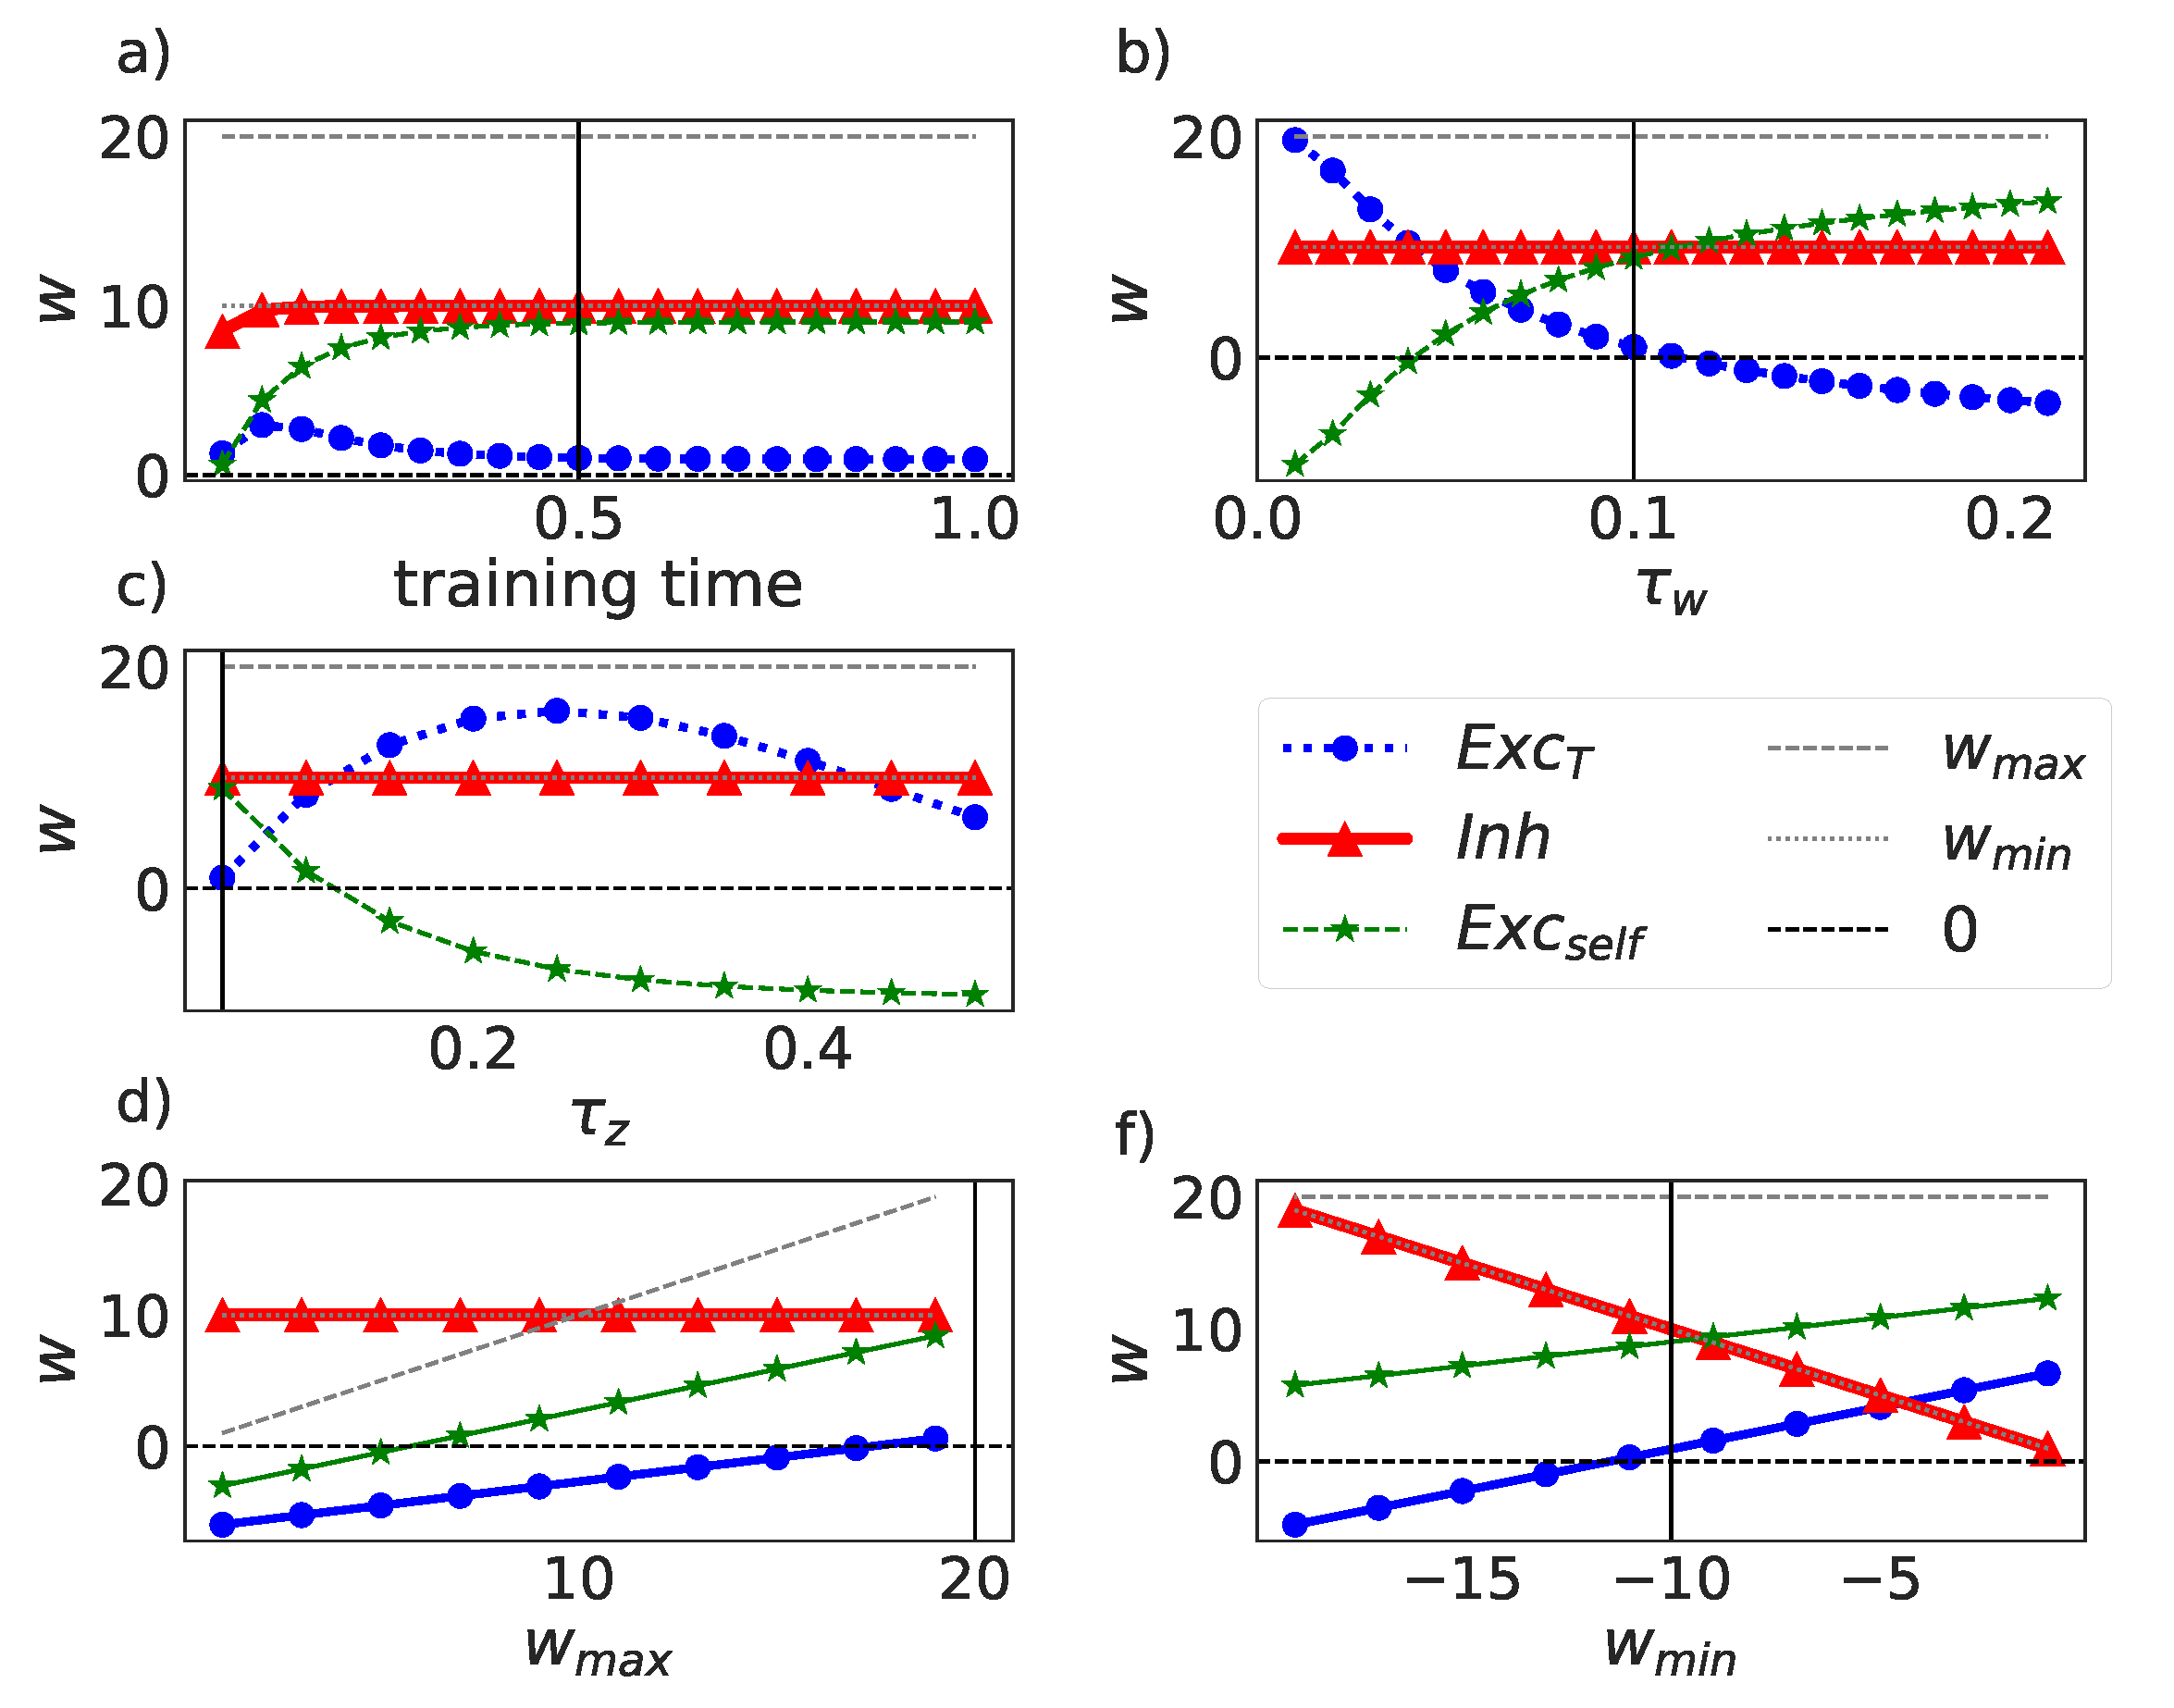
\includegraphics[scale=0.3]{training_rule_quantities_pre_rule_True.eps}
\caption{The dynamics of the learning rule}\label{Fig:learning_quantities_pre}
\end{figure}


\textbf{Training time}
\begin{itemize}
\item  $Exc_{self}$: The longer the training time the longer the filter is activated with itself and therefore it grows. But given that the pre and post filters do not coincide completely in the temporal domain there are negative contributions which prevent this from reaching the saturation value $w_{max}$
\item  $Inh$: In this case the the negative contributions come from the time that the units are not activated together with their counterparts which is most of the time (except in the brief transition period) and therefore the value saturates quickly to $w_{min}$.
\item $Exc_{T}$: In this case what matters is the transition time between two 
\end{itemize} 


\begin{figure}[h!]
\centering
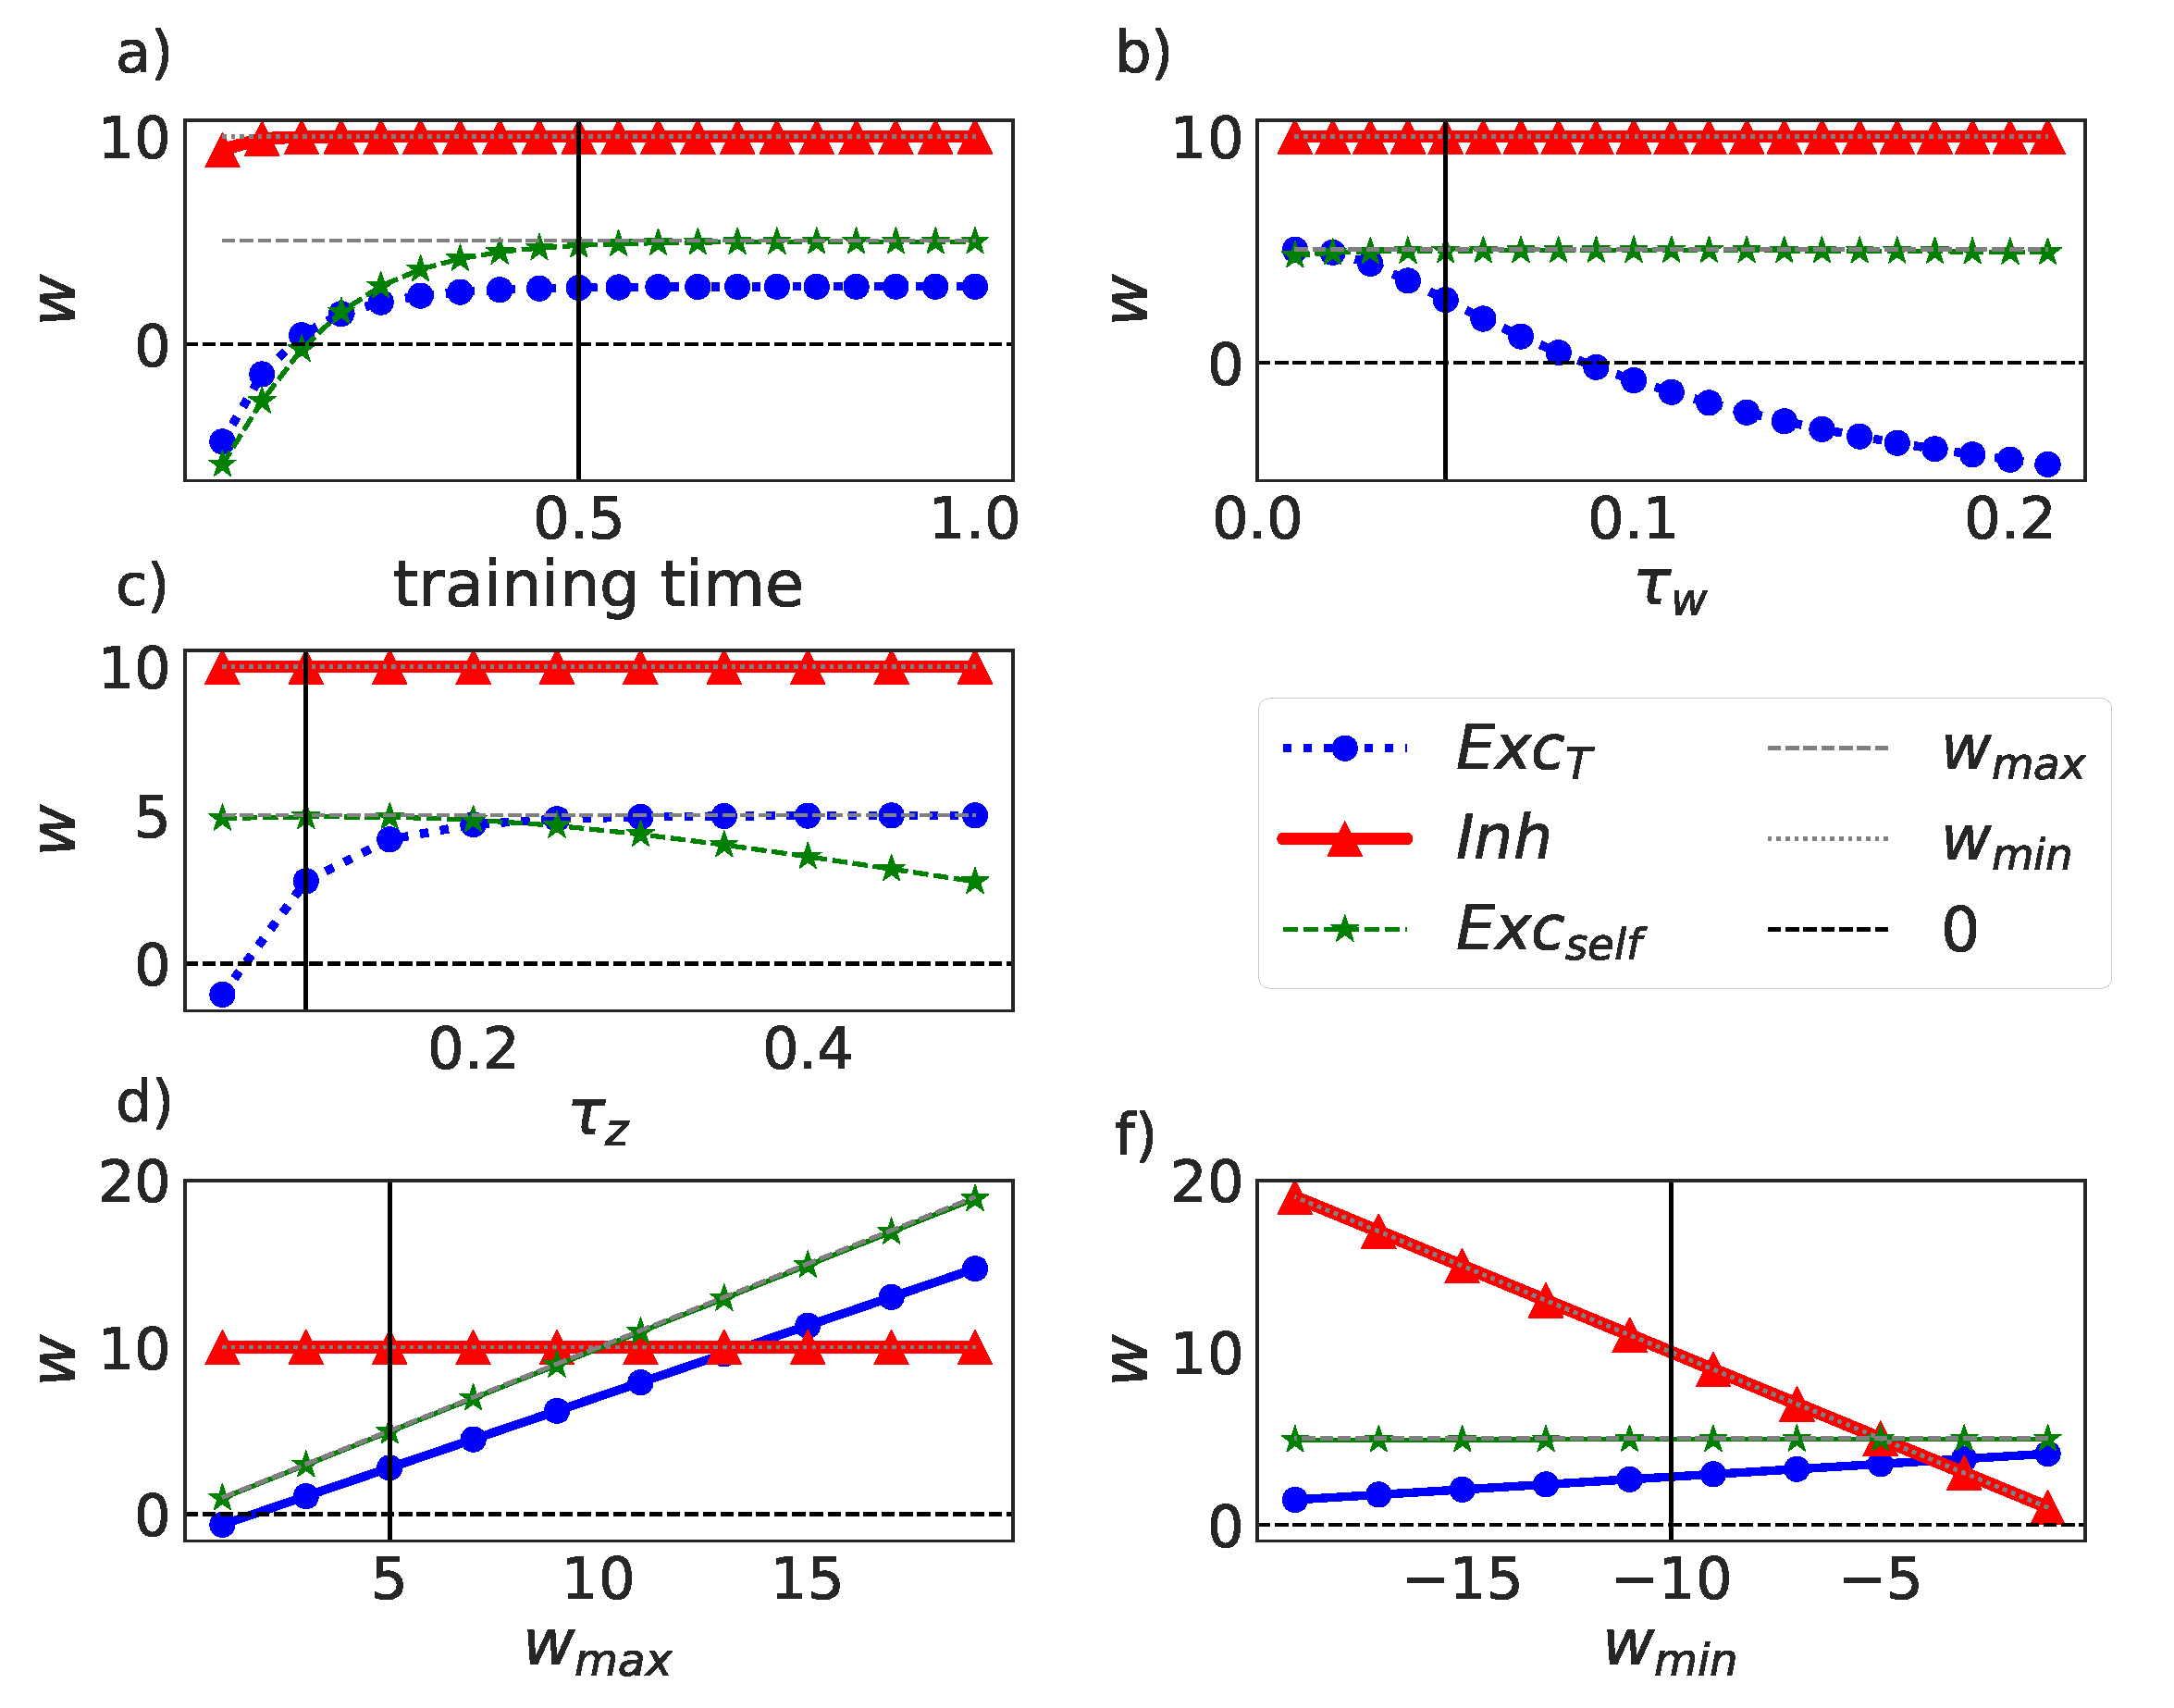
\includegraphics[scale=0.3]{training_rule_quantities_pre_rule_False.eps}
\caption{The dynamics of the learning rule}\label{Fig:learning_quantities_post}
\end{figure}

 
\subsection{Disambiguation}


\section{Discussion}


% ****************************************************************************
% BIBLIOGRAPHY AREA
% ****************************************************************************

\begin{footnotesize}

% IF YOU USE BIBTEX,
% - DELETE THE TEXT BETWEEN THE TWO ABOVE DASHED LINES
% - UNCOMMENT THE NEXT TWO LINES AND REPLACE 'Name_Of_Your_BibFile'

\bibliographystyle{unsrt}
\bibliography{references.bib}

\end{footnotesize}

% ****************************************************************************
% END OF BIBLIOGRAPHY AREA
% ****************************************************************************

\end{document}
